%Beamer class
\documentclass{beamer}

\usepackage[czech]{babel}
\usepackage[utf8]{inputenc}
\usepackage{fontenc}
\usepackage{tgheros}
\usepackage{array}
\usepackage{color}
\usepackage{hyperref}

\usetheme{Antibes}
\usecolortheme{crane}


\title[Instalace KiCAD]{Instalace KiCAD}
\subtitle[KEO] {Konstrukce a realizace elektronických obvodů}
\author[Brejcha]{\texorpdfstring{Michal Brejcha\newline\url{brejcmic@fel.cvut.cz}}{Michal Brejcha}}
\institute[CVUT]{ČVUT v Praze, FEL}
\date[Praha, 2021]{Praha, 2021}

%------------------------------------------------------------------------------
%Konstanty a definice
%------------------------------------------------------------------------------
\newtheorem{myDef}{}
\newcommand{\kicadVersion}{5.1.10.}

\begin{document}
%------------------------------------------------------------------------------
%Uvodni slajd
%------------------------------------------------------------------------------
\frame{\titlepage}

\begin{frame}
\frametitle{Obsah} 
\tableofcontents
\end{frame}

\AtBeginSection[]
{
  \begin{frame}
    \frametitle{Téma}
    \tableofcontents[currentsection]
  \end{frame}
}

%------------------------------------------------------------------------------
%Instalace KiCAD
%------------------------------------------------------------------------------
\section{\texorpdfstring{Instalace KiCAD}{Instalace Kicad}}
%------------------------------------------------------------------------------
	\begin{frame}
    \frametitle{Stažení návrhového systému KiCAD}
		
		\begin{description}
			\item[url:] \url{http://kicad-pcb.org/}
			\item[sekce:] download
		\end{description}
		
		\begin{center}
			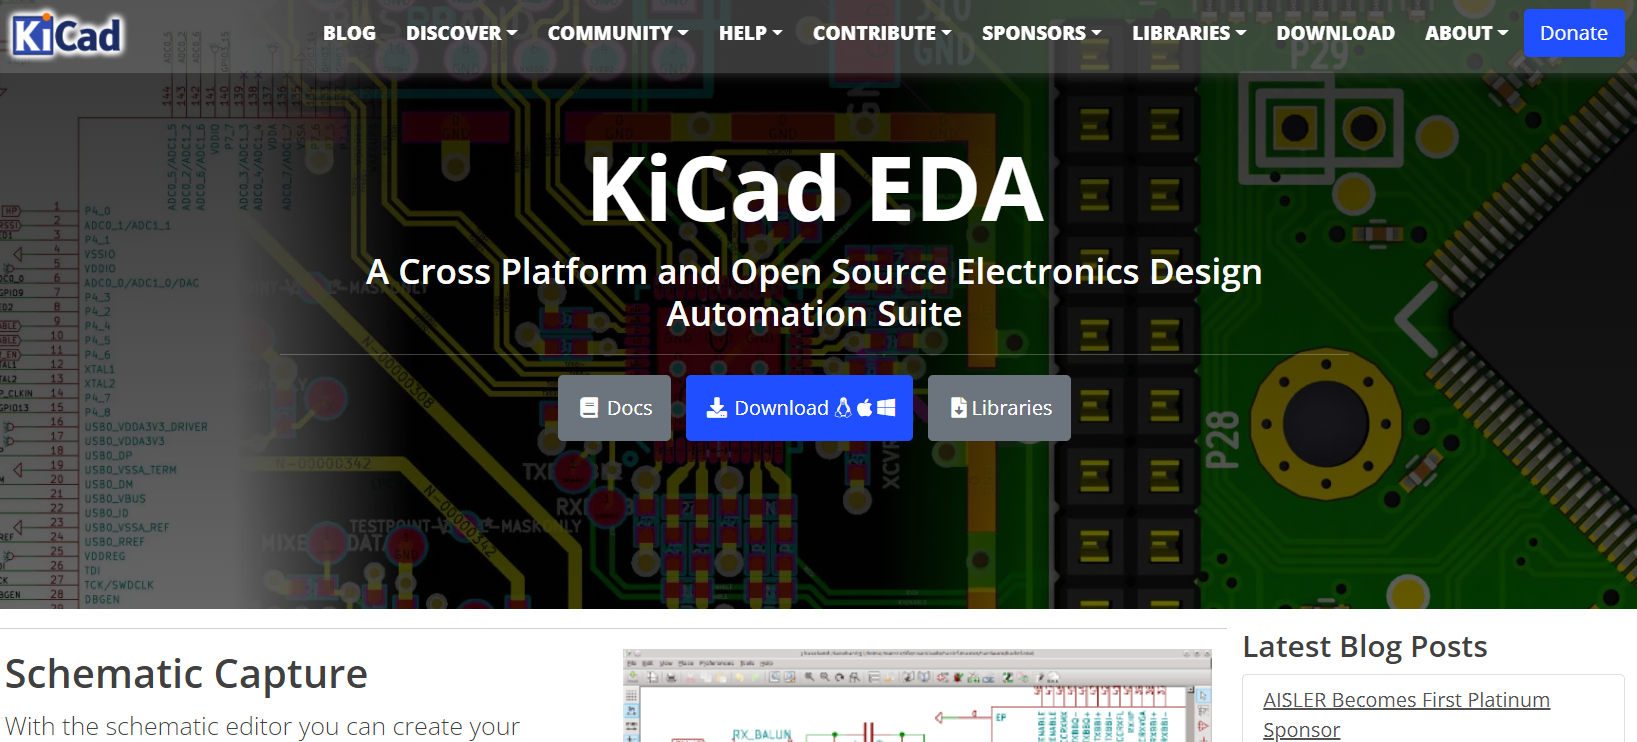
\includegraphics[scale=0.3]{obr/kicad_url.png}
		\end{center}
	\end{frame}
%------------------------------------------------------------------------------
	\begin{frame}
    \frametitle{Výběr operačního systému}
		\small
		\begin{itemize}
			\item instalace windows již obsahuje všechny knihovny
			\item v případě ubuntu je třeba přidat ppa, aby se stáhla poslední verze KiCAD \kicadVersion\
		\end{itemize}
		
		\begin{center}
			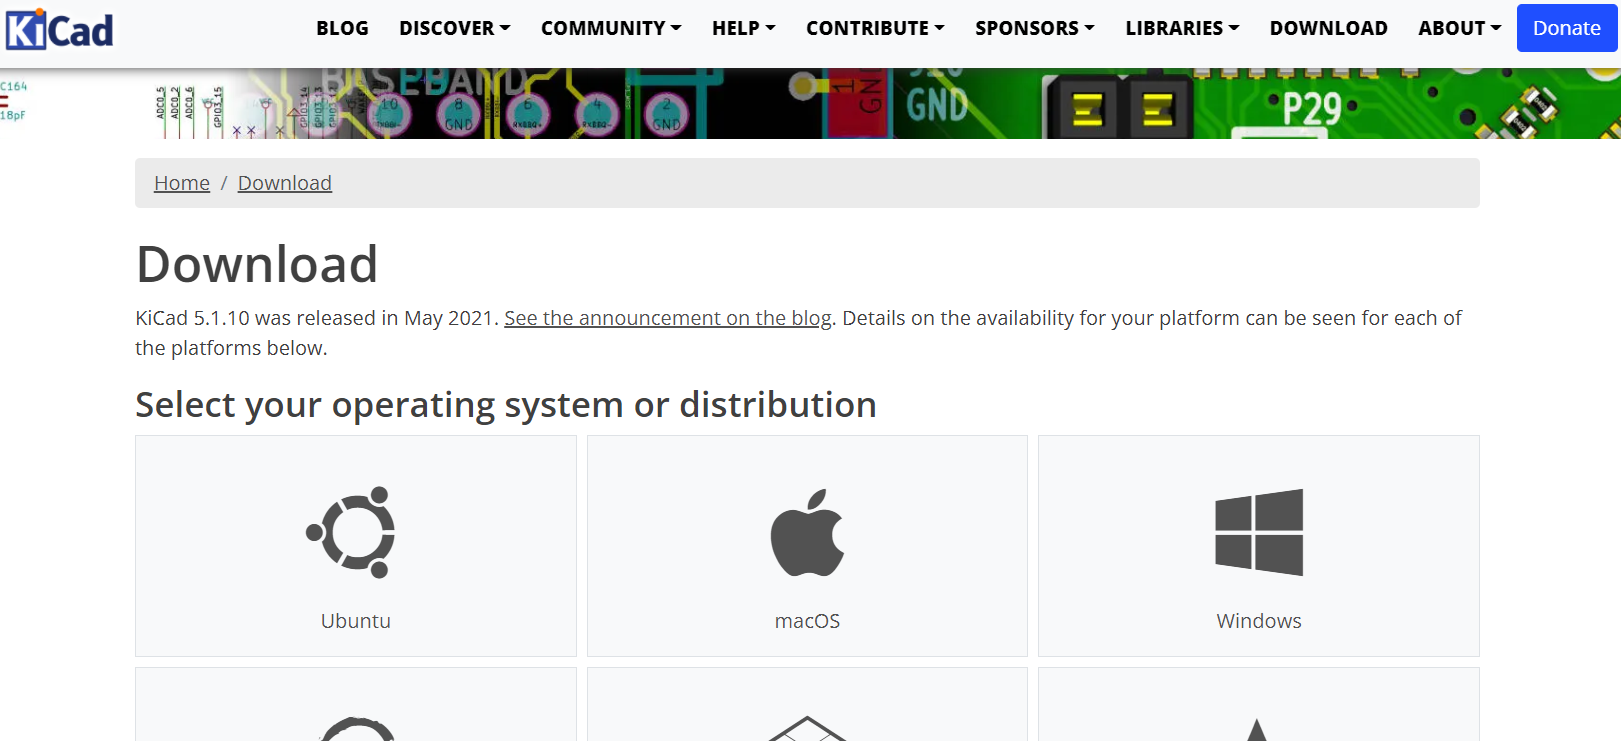
\includegraphics[scale=0.3]{obr/kicad_dwnld.png}
		\end{center}
	\end{frame}
%------------------------------------------------------------------------------
	\begin{frame}
    \frametitle{Stažení instalačního souboru}
		\small
		\begin{itemize}
			\item stáhnout aktuální stabilní verzi \kicadVersion\
		\end{itemize}
		
		\begin{center}
			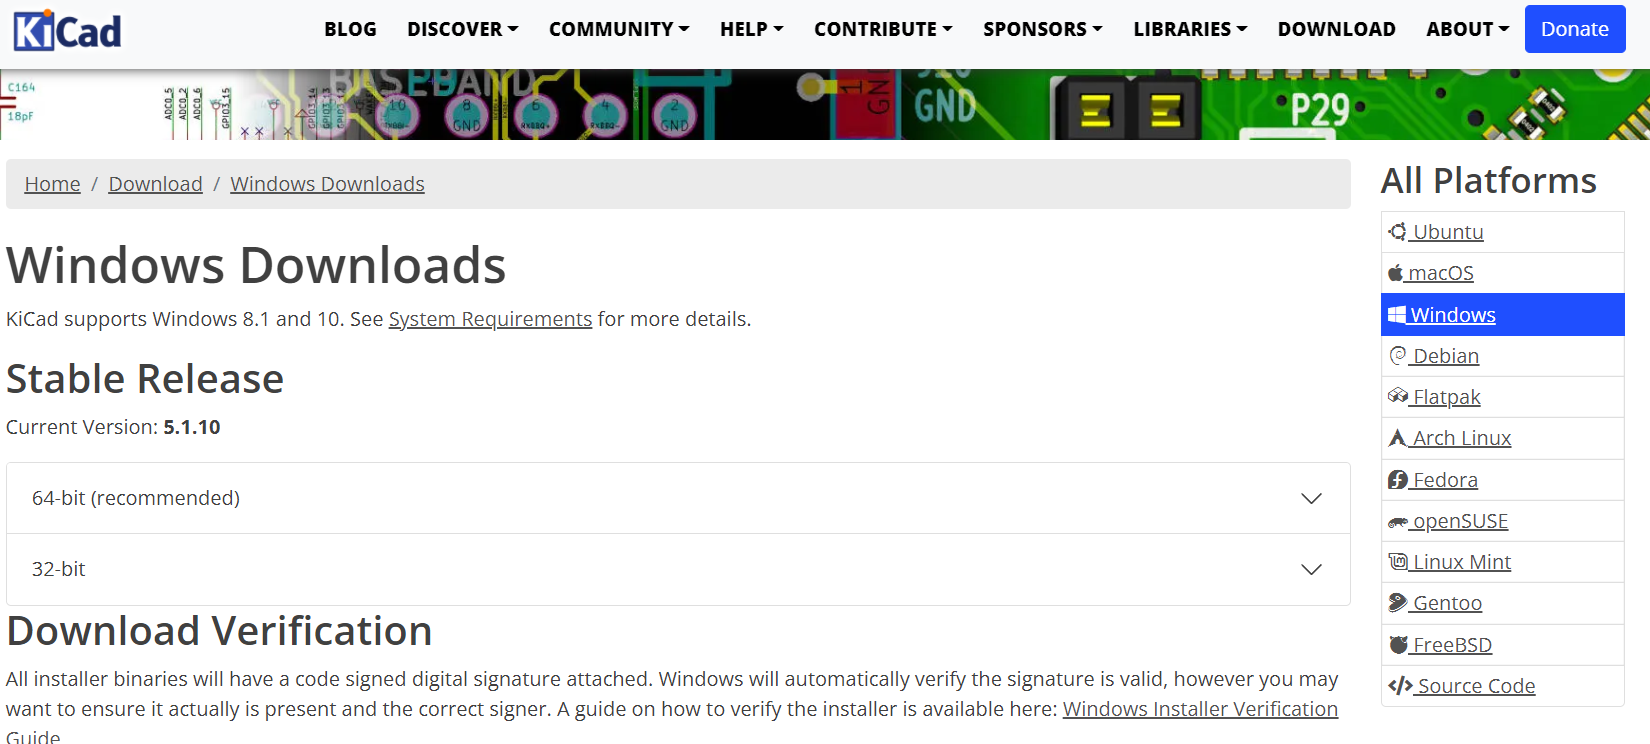
\includegraphics[scale=0.3]{obr/kicad_stbv.png}
		\end{center}
	\end{frame}
%------------------------------------------------------------------------------
	\begin{frame}
    \frametitle{Instalace - Windows}
    	\textbf{Vhodný návod v podobě videa na youtube:} \url{https://www.youtube.com/watch?v=Cu2VlXy-PzM} \\~\\
    	
    	\textbf{Poznámky:}
		\begin{enumerate}
			\item poklepat na stažený instalační soubor
			\item v prvním okně zvolit další,
			\item vše ve volbě součástí nechat zaškrtnuté, jen v případě jazyků zrušit vše kromě češtiny a angličtiny,
			\item zvolit další a přejít do nastavení umístění, umístění doporučuji nechat původní předepsané,
			\item zvolit další a nechat proběhnout instalaci
		\end{enumerate}
		
	\end{frame}
%------------------------------------------------------------------------------
	\begin{frame}
    \frametitle{Průběh instalace}
		\begin{center}
			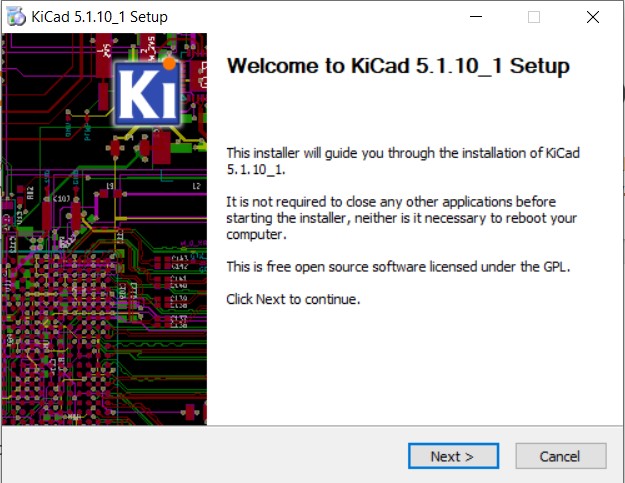
\includegraphics[scale=0.5]{obr/kicad_inst1.png}
		\end{center}
		
		\begin{itemize}
			\item Zde zvolte \uv{Next}.
		\end{itemize}
	\end{frame}
%------------------------------------------------------------------------------
	\begin{frame}
    \frametitle{Průběh instalace}
		\begin{center}
			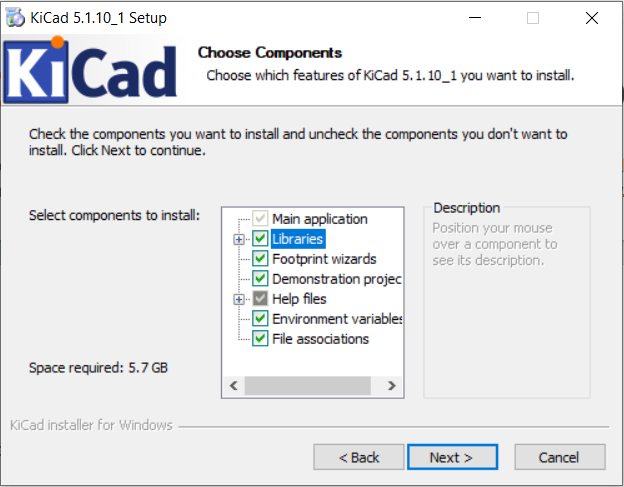
\includegraphics[scale=0.5]{obr/kicad_inst2.png}
		\end{center}
		
		\begin{itemize}
			\item Vše nechte kromě \uv{Help files} zaškrtnuté, v \uv{Help files} ponechte jen \uv{English}.
		\end{itemize}
	\end{frame}
%------------------------------------------------------------------------------
	\begin{frame}
    \frametitle{Průběh instalace}
		\begin{center}
			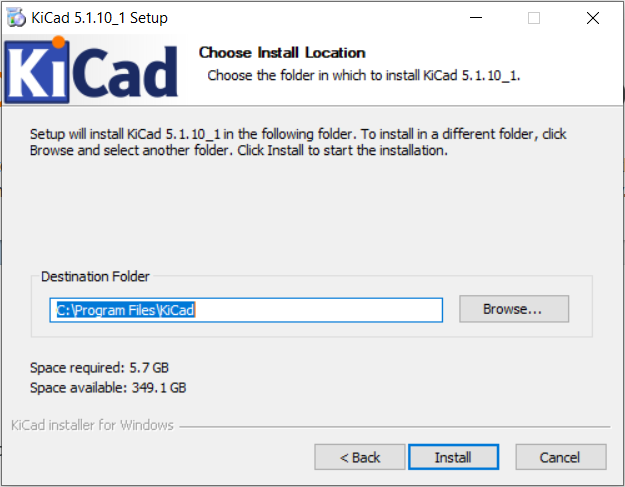
\includegraphics[scale=0.5]{obr/kicad_inst3.png}
		\end{center}
		
		\begin{itemize}
			\item Nechte původní cestu a zvolte \uv{Install}
		\end{itemize}
	\end{frame}
%------------------------------------------------------------------------------
	\begin{frame}
    \frametitle{Průběh instalace}
		\begin{center}
			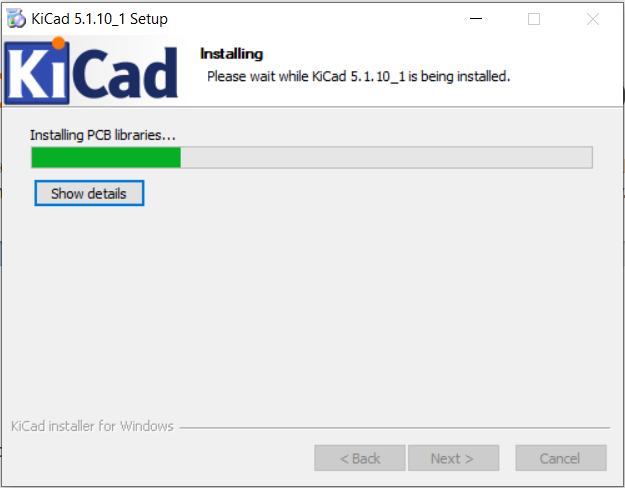
\includegraphics[scale=0.5]{obr/kicad_inst4.png}
		\end{center}
		
		\begin{itemize}
			\item Vyčkejte do konce instalace.
		\end{itemize}
	\end{frame}
%------------------------------------------------------------------------------
	\begin{frame}
    \frametitle{Průběh instalace}
		\begin{center}
			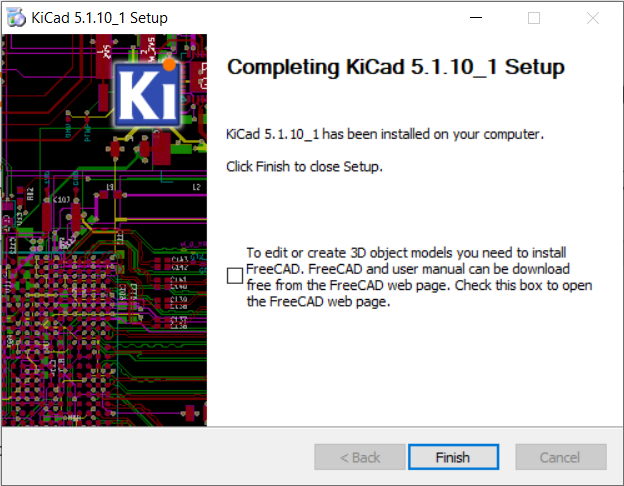
\includegraphics[scale=0.5]{obr/kicad_inst5.png}
		\end{center}
		
		\begin{itemize}
			\item Potvrďte dokončení instalace, zaškrtávátko se týká 3D modelů součástek, které v předmětu KEO dělat nebudete.
		\end{itemize}
	\end{frame}
%------------------------------------------------------------------------------
	\begin{frame}
    \frametitle{První spuštění}
    \small
    	Po instalaci se v nabídce start objeví několik nových programů:
      \begin{tabular}{ m{6cm} m{2cm} }
         \begin{itemize}
           \item \textbf{KiCad}
           \item Eeschema
           \item Pcbnew
           \item Gerbview
           \item PCB calculator
           \item Pagelayout editor
         \end{itemize}
         & 
        \begin{minipage}{\textwidth}
          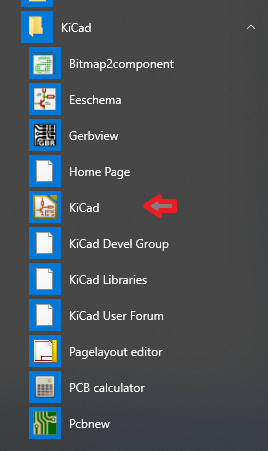
\includegraphics[scale=0.3]{obr/nabStart.png}
        \end{minipage}
				\vspace{0.2cm}
      \end{tabular} 
   
  Vždy spouštíme KiCad, chceme pracovat s projekty.
	\end{frame}
%------------------------------------------------------------------------------
	\begin{frame}
    \frametitle{První spuštění}
    \small
    Při prvním spuštění se program dotáže na tvorbu a umístění souboru \textit{\textbf{sym-lib-table}}. V tomto případě nechte doporučenou první volbu.
    \begin{center}
			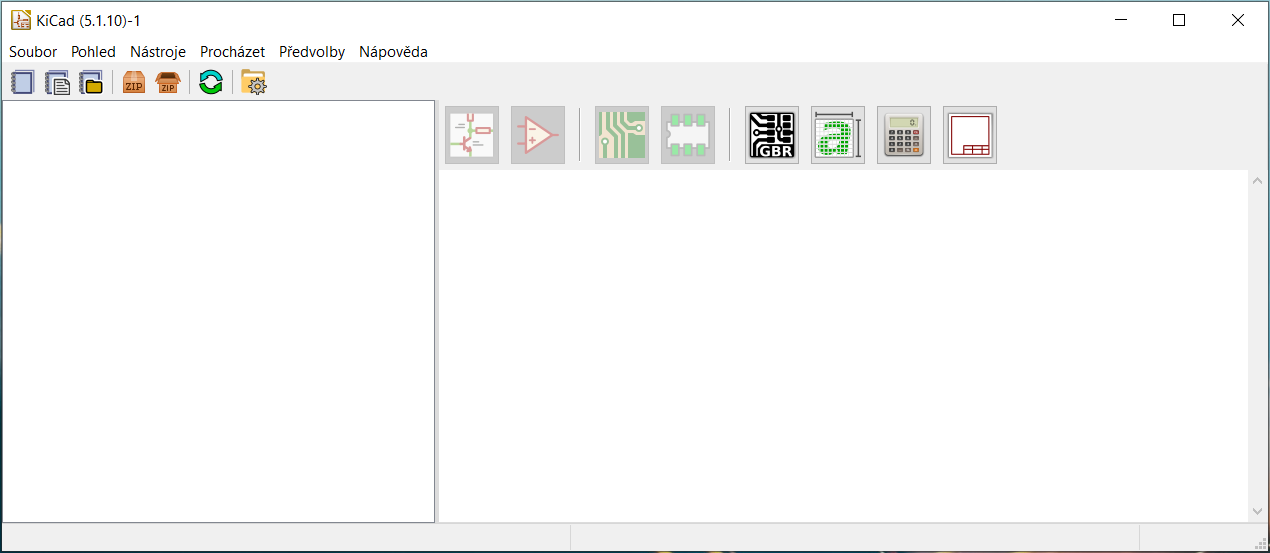
\includegraphics[scale=0.4]{obr/kicad_nabidka.png}
		\end{center}
	\end{frame}
%------------------------------------------------------------------------------

%Stazeni knihoven
%------------------------------------------------------------------------------
\section{\texorpdfstring{Stažení knihoven}{Stazeni knihoven}}
%------------------------------------------------------------------------------
	\begin{frame}
    \frametitle{Oficiální knihovny}
   
    \textcolor{red}{Počáteční knihovny} KiCAD, které jsou součástí instalace, jsou rozdílné od oficiálních knihoven a také \textcolor{red}{jsou méně obsáhlé}.
    \vspace{0.5 cm}
		
		\textbf{Stažení oficiálních knihoven}:
		\begin{itemize}
			\item[\textcolor{green}{\textbf{+}}] Jsou spravovány a aktualizovány komunitou,
			\item[\textcolor{green}{\textbf{+}}] s GIT je lze snadno aktualizovat,
			\item[\textcolor{green}{\textbf{+}}] mají mnohem více prvků než původní knihovny po instalaci.
			\item[\textcolor{red}{\textbf{\text{--}}}] Pro jejich funkci je třeba v programu přiřadit cesty.
		\end{itemize}
	\end{frame}
%------------------------------------------------------------------------------
	\begin{frame}
    \frametitle{Úložiště oficiálních knihoven}

    \begin{center}
			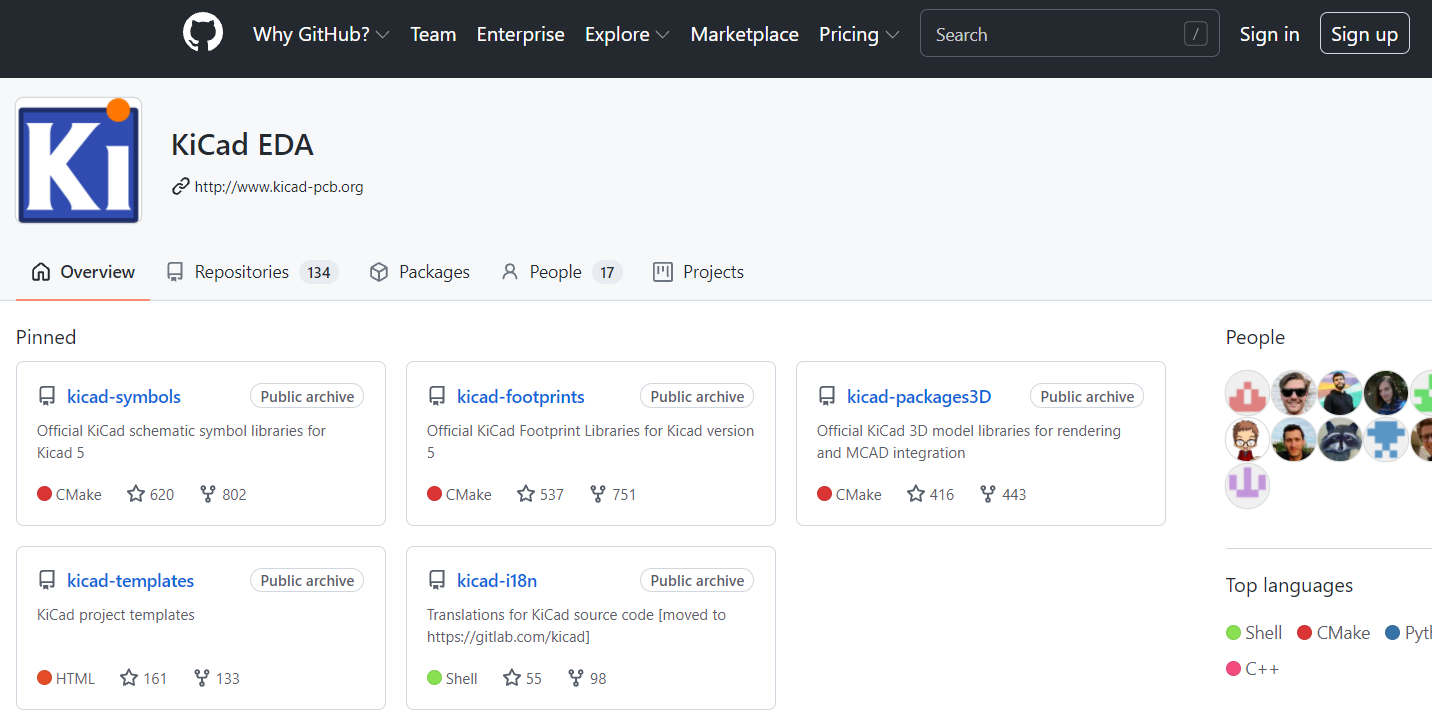
\includegraphics[scale=0.3]{obr/github_lib1.png}
		\end{center}
		
		Adresa: \url{https://github.com/KiCad}
		
		Potřebujeme: kicad-symbols, kicad-footprints
		
	\end{frame}
%------------------------------------------------------------------------------
	\begin{frame}
    \frametitle{Stažení}

    \begin{center}
			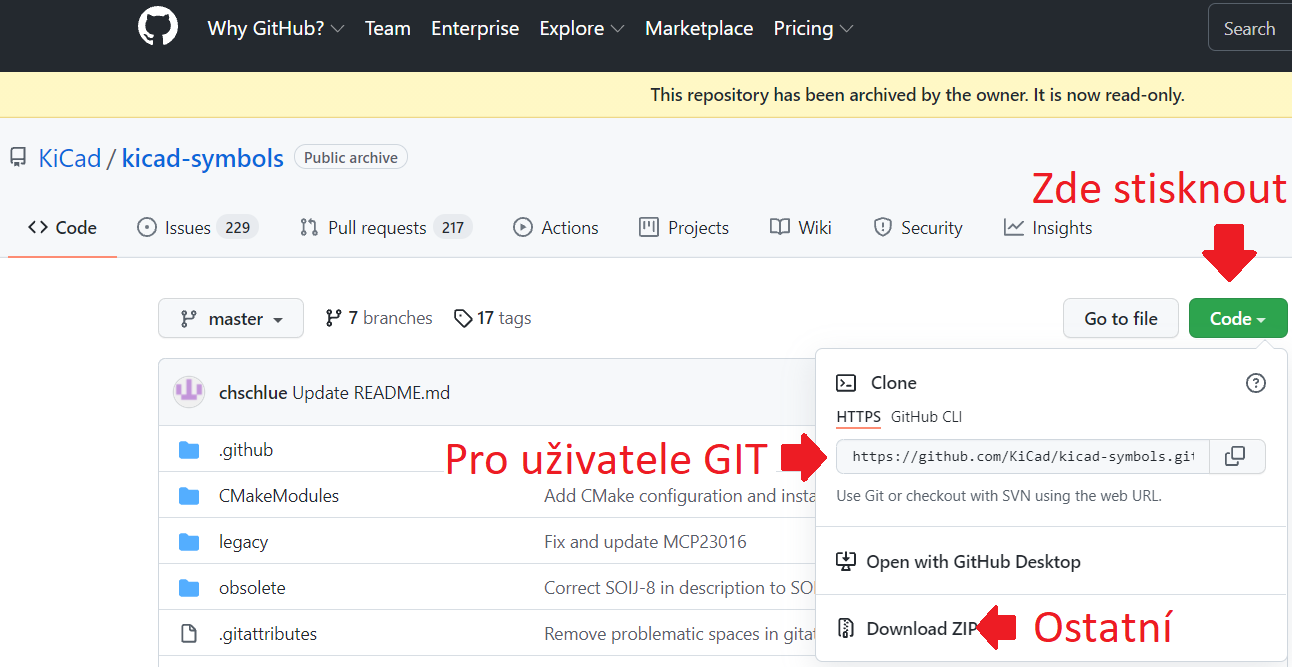
\includegraphics[scale=0.3]{obr/github_lib2.png}
		\end{center}
		
		\begin{itemize}
			\item Uživatelé git mohou klonovat, ostatní stahují soubor zip.
		\end{itemize}
		
	\end{frame}
%------------------------------------------------------------------------------
	\begin{frame}
    \frametitle{Stažení}

    \begin{center}
			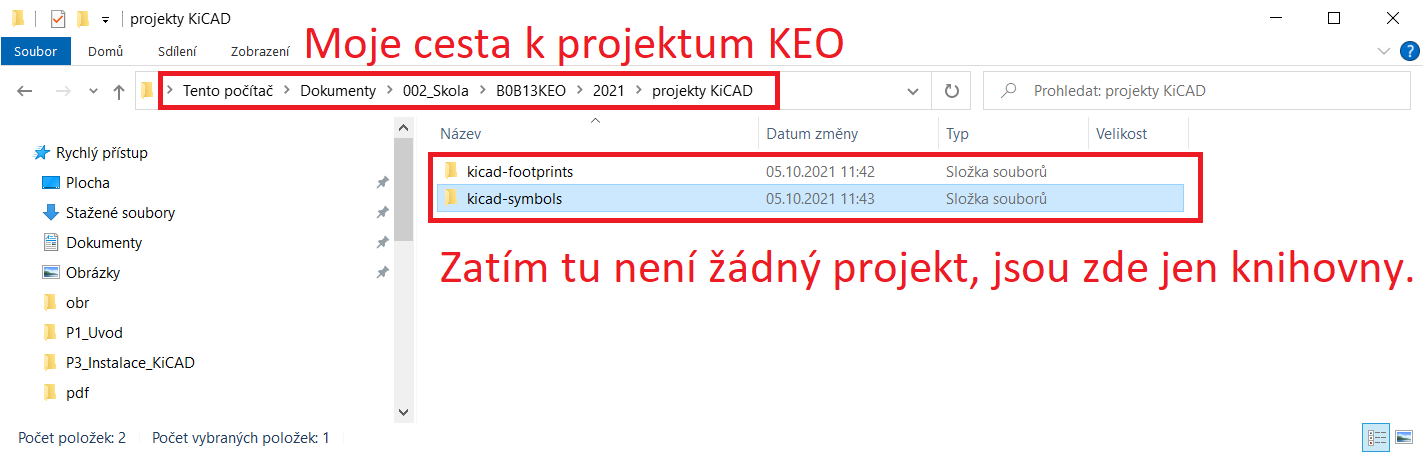
\includegraphics[scale=0.35]{obr/proj_lib1.png}
		\end{center}
	
		\begin{itemize}
			\item Cílovým adresářem pro rozbalení nebo klonování se předpokládá adresář s KiCAD projekty.
		\end{itemize}
		
	\end{frame}
%------------------------------------------------------------------------------
	\begin{frame}
    \frametitle{Co bude příště}
	
		Přednáška a cvičení s výkladem pro kreslení v editoru schémat:
		\begin{itemize}
			\item Založení projektu,
			\item přidání knihoven,
			\item kreslení schéma, výběr součástek apod.
			\item kontrola zapojení,
			\item přiřazení pouzder.
		\end{itemize}
		Obě hodiny budou v počítačové učebně \textbf{T2:C4-264}. Nicméně, je možné pracovat i na vlastním notebooku. 
	\end{frame}
%------------------------------------------------------------------------------
\end{document}